% main.tex — SoK: From Assistive to Autonomous (CP3 assembly)
\documentclass[conference,compsoc]{IEEEtran}
\usepackage[T1]{fontenc}
\usepackage[utf8]{inputenc}
\usepackage{cite}
\usepackage{tikz}
\usetikzlibrary{arrows.meta,bending,calc,shapes.geometric}
\usepackage{booktabs}
\usepackage{caption}
\usepackage{xurl}
\usepackage{balance}

\newcommand{\Bset}[1]{\ensuremath{\{#1\}}}

\begin{document}

\title{SoK: From Assistive to Autonomous --- The Co-Evolution of\\ LLM-Driven Vulnerability Discovery, Exploitation and Patching}

\author{\IEEEauthorblockN{Anonymous Submission}\\
\IEEEauthorblockA{Double-blind review copy}}

\maketitle

\begin{abstract}
Large language models have moved from answering security questions to executing security work.
We systematize this transition across a 36-record multi-stream corpus --- academic literature,
competition and industrial documents, and registry records --- using two orthogonal axes: a
decision-authority gradient (A0 assistive to A3 autonomous production hunter), assigned only by
documented behavior under the rule that claims are graded by their weakest missing condition,
and the offense/defense loop positions B1--B4. Fourteen in-window records bear autonomy
classifications: pipeline automation (A1) already operates at ecosystem scale; task agents (A2)
appear in seeded production research, entry-point-assisted auditing, black-box platform
operation, and the DARPA AI Cyber Challenge's fully autonomous scored rounds; no included
evidence meets our operational definition of A3. We further grade offense$\leftrightarrow$
defense coupling, documenting an explicit cross-program edge (Project Zero's SQLite campaign
citing AIxCC as inspiration) while declining field-wide causal claims, and we systematize
evaluation validity as a measured constraint: information conditions swing headline exploitation
rates twelve-fold, dataset reconstruction collapses detection performance, and proof-of-
vulnerability oracles admit documented mitigation gaming. We close with a falsifier-specified
roadmap --- from autonomy-versus-scale ablations to decision-impact audits --- for converting an
increasingly autonomous practice into an increasingly verifiable one.
\end{abstract}

% sections/01-introduction.tex
\section{Introduction}
\label{sec:intro}

Between 2024 and 2026, vulnerability discovery, exploitation, and patching acquired a new
subject: software systems in which large language models select and execute security-relevant
actions. Google reported an agent finding an exploitable memory-safety zero-day in SQLite that
150 CPU-hours of AFL could not rediscover~\cite{bigsleep2024naptime}; a commercial agent
briefly held the top US position on a major bug-bounty platform~\cite{xbowtop12025}; a
government challenge scored seven fully autonomous systems on finding, proving, and patching
vulnerabilities in open-source software~\cite{darparesults2025,r7sokaixcc2026}; and Anthropic
reported an intrusion campaign whose execution was 80--90\% autonomous~\cite{anthropicgtg2025}.
These events are connected neither by a shared benchmark nor by a shared metric, which is
precisely why existing surveys cannot answer the questions they raise.

\subsection{The Empirical Problem}
Three difficulties block straightforward assessment. First, \emph{unit confusion}: results are
reported about models (benchmark pass rates), pipelines (fuzz-target generation), agents
(tool-using loops), and organizations (leaderboard ranks) as if commensurable. Second,
\emph{loop fragmentation}: discovery, validation, and repair are evaluated separately even when
the deployed systems integrate them. Third, \emph{validity opacity}: headline numbers travel
without the information conditions, label provenance, or adjudication rules that produced them
--- GPT-4-based agents exploited 87\% of one-day CVEs when given their descriptions and 7\%
when not~\cite{fang2024agents}, yet the qualified number is the one usually quoted.

\subsection{Our Approach}
We build a PRISMA-grounded, multi-stream evidence base (academic literature; competition and
industrial documents; registry records) and classify every record on two orthogonal axes:
a \emph{decision-authority} gradient A0--A3, assigned strictly by documented behavior ---
``who chooses the next action?'' --- with autonomy claims graded by their weakest missing
condition; and the offense/defense loop positions B1--B4, recorded as sets for systems spanning
phases. Fourteen in-window records bear autonomy classifications; the remaining 22 provide
context, validity evidence, loop-transition documentation, or related-work positioning, and we
keep the distinction explicit throughout.

\subsection{Contributions}
\textbf{C1.} An autonomy$\times$loop taxonomy applied record-by-record with published
behavioral evidence (Secs.~\ref{sec:framework}, \ref{sec:discovery}; Fig.~\ref{fig:abmap}).
\textbf{C2.} An evidence-graded analysis of offense$\leftrightarrow$defense coupling, including
a documented cross-program causal edge from the AIxCC competition to Project Zero's research
program (Sec.~\ref{sec:coevolution}). \textbf{C3.} A systematization of evaluation-validity
failures as measurable phenomena, with a five-part contamination-control protocol
(Sec.~\ref{sec:validity}). \textbf{C4.} A falsifier-specified experimental roadmap
(Sec.~\ref{sec:roadmap}).

\subsection{Insights}
\textbf{I1.} Evaluation, deployment, and discourse increasingly measure progress in terms of
agentic autonomy rather than model capability alone; whether this reflects a corresponding
shift in underlying capability remains unresolved. \textbf{I2.} Multiple documented
offense$\leftrightarrow$defense coupling edges exist --- including one explicit cross-program
inspiration --- but the evidence does not establish field-wide causal co-evolution.
\textbf{I3.} Evaluation validity is a binding methodological constraint on what this field can
claim to know.

\subsection{Scope}
We cover January 2024--June 2026, with pre-2024 work as background only. We classify
\emph{documented behavior}, not marketing; we distinguish vendor-reported from independently
verified results everywhere; and we found it necessary to state plainly that no included
evidence met our operational definition of an autonomous production hunter (A3). We explicitly
exclude the AgentFlow paper~\cite{agentless2024} from our comparison and analysis, as its
focus on multi-agent orchestration for code generation falls outside our vulnerability discovery,
exploitation, and patching scope.

% sections/02-related-work.tex — background + R1–R7 differentiation + positioning table.
\section{Background and Related Work}
\label{sec:related}

\subsection{Background}
Three technical threads meet in this paper. \emph{Code LLMs} provide the reasoning substrate;
their security-relevant evaluations began with secure-coding benchmarks~\cite{csev12023} and
matured into risk suites probing cyberattack helpfulness~\cite{csev22024,csev32024}.
\emph{Vulnerability detection} supplies B1's evaluation layer, where PrimeVul demonstrated that
label noise and temporal leakage had inflated a generation of results~\cite{primevul2024},
a critique systematized by Risse and B\"ohme~\cite{rissebohme2024}. \emph{Interactive
agent harnesses} descend from execution-feedback benchmarks such as InterCode-CTF
(pre-2024 background)~\cite{intercode2023} through NYU CTF Bench~\cite{nyuctfbench2024} and
Cybench~\cite{cybench2024}. PentestGPT established the penetration-testing tree (PTT) as a
planning data structure for LLM-empowered automated penetration testing, demonstrating that
domain-grounded agent architectures outperform raw prompting on real-world
targets~\cite{pentestgpt2024}. Finally, the Model Context Protocol ecosystem --- measured at
scale for server-side insecurity~\cite{mcpfirstlook2025} and analyzed for tool-poisoning,
spec-level, and governance risks~\cite{mcppoisoning2026,mcpspec2026,mcpgovernance2025} ---
supplies the tool-integration substrate on which A2 autonomy operates.

\subsection{Systematizations We Position Against}
Table~\ref{tab:positioning} differentiates the seven closest prior efforts. R1's SLR mapped
300+ LLM$\times$security works but closed before the agentic turn~\cite{zhang2024when}; R2
covers detection-to-remediation with no exploitation axis~\cite{r2slr2024remediation}; R3 ---
the closest survey chronologically --- organizes pentesting only, treats ``co-evolution'' as an
architecture--benchmark relationship internal to that subfield, and excludes competition-grade
systems by corpus design; it is also outside our window (July 2026), so we use it as a
comparator, not migration evidence~\cite{r3survey2026pentest}. R4 is detection-centric within
software security~\cite{sheng2025csur}. R5 systematizes the security of agent systems ---
agents as attack surface --- whereas our subject is agents as operators of the vulnerability
loop~\cite{r5usenix26agentic}. R6's TOSEM SLR contributes 263 detection studies through
November 2025 but no offense axis and no industrial track~\cite{tosemslr2026}. R7, the AIxCC
systematization, is our most important predecessor: we cite-and-exceed it by placing CRSs on
an autonomy gradient, extending analysis to post-competition redeployment (B4), and adding the
validity critique its design-focused treatment does not attempt~\cite{r7sokaixcc2026}.

\begin{table}[t]
\centering\scriptsize
\caption{Positioning against prior systematizations. C=covered, P=partial, A=absent.}
\label{tab:positioning}
\resizebox{\columnwidth}{!}{%
\begin{tabular}{lcccccc}
\hline
Work & Window-end & Offense & Defense & Loop & Comp./industr. & Contamination\\
\hline
R1 \cite{zhang2024when}        & Aug'24 & P & C & A & A & P\\
R2 \cite{r2slr2024remediation} & Dec'24 & A & C & A & A & P\\
R3 \cite{r3survey2026pentest}  & Jul'26$^{\dagger}$ & C & P & P (intra-pentest) & A & A\\
R4 \cite{sheng2025csur}        & '25    & A & C & A & A & A\\
R5 \cite{r5usenix26agentic}    & '26    & P & P & A & P & A\\
R6 \cite{tosemslr2026}         & Nov'25 & A & C & A & P (repo) & P\\
R7 \cite{r7sokaixcc2026}       & Aug'26 & C & C & P & C & A\\
Ours                           & Jun'26 & C & C & C (graded) & C & C (measured+protocol)\\
\hline
\multicolumn{7}{l}{$^{\dagger}$Out-of-window comparator; discussed in related work only.}
\end{tabular}}
\end{table}

\subsection{What Remains Uncovered}
No prior systematization joins (i) an autonomy gradient applied to documented behavior across
academic, competition, and industrial streams; (ii) loop integration including post-competition
redeployment; and (iii) evaluation validity as a measured, protocol-addressable variable. That
conjunction is this paper's contribution.

% sections/03-methodology.tex — PRISMA multi-stream methodology (spec §5).
\section{Methodology}
\label{sec:method}

\subsection{Study Design}
We conduct a PRISMA-grounded systematization with one deliberate structural change: because the
subject spans academic papers, competition artifacts, vendor disclosures, and registry records,
we maintain \textbf{three evidence streams} rather than forcing all material through a single
review flow. Stream~A (academic literature) follows the classical funnel; Stream~B
(competition/industrial/foundation documents) follows targeted acquisition with quote-level
extraction; Stream~C (registry records, e.g., NVD entries) follows existence verification. The
streams are reported separately and only summed at the top level.

\subsection{Search Strategy}
Stream~A searches used arXiv boolean queries (eight formulations over ``large language model''
/ ``language model'' / ``LLM agent'' crossed with vulnerability discovery, detection,
penetration testing, CTF, exploit, program repair, cyber reasoning system; total 973 raw hits)
and four DBLP queries (214 hits), filtered to January~2024--June~2026 submission dates.
Publisher APIs were unavailable; IEEE/ACM/USENIX coverage came from official indexes and
citation chaining, a limitation we return to below. Streams B/C used targeted retrieval:
official program pages, team/vendor blogs, foundation retrospectives, and NVD. The complete
query log with per-query hit counts is Appendix~B.

% figures/prisma-flow.tex — F1: multi-stream PRISMA flow (layout-aligned revision)
% Counts from prisma-counts.csv / search-log.md (frozen CP1-final numbers).
\begin{figure}[t]
\centering
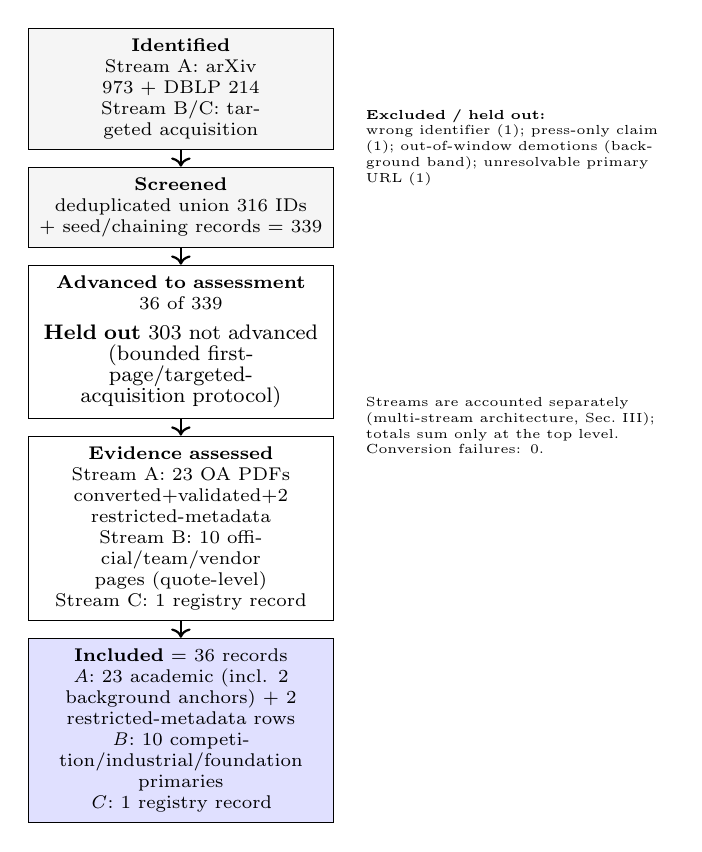
\begin{tikzpicture}[
  box/.style={draw,align=center,font=\scriptsize,inner sep=4pt,minimum height=0.85cm,text width=3.8cm},
  arr/.style={->,thick}, scale=0.95,transform shape]
\node[box,fill=gray!8] (id) at (0,0)
 {\textbf{Identified}\\ Stream A: arXiv 973 + DBLP 214\\ Stream B/C: targeted acquisition};
\node[box,fill=gray!8,anchor=north] (scr) at ($(id.south)+(0,-0.22)$)
 {\textbf{Screened}\\ deduplicated union 316 IDs\\ $+$ seed/chaining records $=$ 339};
\node[box,anchor=north] (held) at ($(scr.south)+(0,-0.22)$)
 {\textbf{Advanced to assessment}\\ 36 of 339\\[2pt]
 \footnotesize\textbf{Held out} 303 not advanced\\
 (bounded first-page/targeted-acquisition protocol)};
\node[box,anchor=north] (ftx) at ($(held.south)+(0,-0.22)$)
 {\textbf{Evidence assessed}\\ Stream A: 23 OA PDFs converted$+$validated$+$2 restricted-metadata\\
  Stream B: 10 official/team/vendor pages (quote-level)\\ Stream C: 1 registry record};
\node[box,fill=blue!12,anchor=north] (inc) at ($(ftx.south)+(0,-0.22)$)
 {\textbf{Included} $=$ 36 records\\
  \emph{A}: 23 academic (incl. 2 background anchors) $+$ 2 restricted-metadata rows\\
  \emph{B}: 10 competition/industrial/foundation primaries\\
  \emph{C}: 1 registry record};
\draw[arr] (id.south)--(scr.north); \draw[arr] (scr.south)--(held.north); \draw[arr] (held.south)--(ftx.north); \draw[arr] (ftx.south)--(inc.north);
\node[font=\tiny,anchor=west,text width=4.0cm] at (2.35,-0.78)
 {\textbf{Excluded / held out:}\\ wrong identifier (1); press-only claim (1); out-of-window demotions
  (background band); unresolvable primary URL (1)};
\node[font=\tiny,anchor=west,text width=4.0cm] at (2.35,-4.5)
 {Streams are accounted separately (multi-stream architecture, Sec.~III); totals sum only at the top level.
  Conversion failures: 0.};
\end{tikzpicture}
\caption{Multi-stream PRISMA flow. Unlike single-corpus reviews, evidence here arrives in
three streams with different verification obligations; each stream keeps its own denominators and only the included set is summed (36 records). Full query strings, per-query hit counts, exclusion reasons, and saturation tests appear in Appendices~\ref{app:search}
and the repository artifacts.}
\label{fig:prisma}
\end{figure}


\subsection{Selection and Corpus}
Screening operated on a deduplicated pool (316 distinct arXiv IDs plus seed/chaining records).
Inclusion required peer-reviewed status, influential preprint status, or documented-system
evidence relevant to at least one framework cell. The final corpus holds \textbf{36 records}:
23 academic works with full texts converted and validated locally, 2 restricted-access
surveys positioned via verified metadata, 10 competition/industrial primaries with verbatim
quote extraction, and 1 registry record. Four candidate records were excluded (wrong
identifier, press-only claims, out-of-window scope, unresolvable primary URL). Saturation was
tested non-circularly across six novelty axes (new systems, new loop mechanisms, new validity
problems, contradictions, new industrial evidence, negative results); two consecutive passes
without axis-level novelty stopped inclusion.

\subsection{Quality Rubric and Evidence Classes}
Each record carries reproducibility, baseline-rigor, and artifact-availability scores (0--3),
plus evidence class (benchmark, controlled experiment, production-network experiment,
competition, production discovery, incident report, measurement, registry), unit type, access
status, and provenance type (PDF+TXT, HTML-extract, metadata-only). Vendor-reported statistics
are labeled CLAIMED regardless of source authority; third-party reproduction passes are marked
as such.

\subsection{Classification Protocol}
Autonomy (A0--A3) is assigned by the decision-authority test --- who chooses the next action? ---
with A3 additionally requiring independent planning, execution, validation, and reporting in
environment class E2 (production or production-like external targets; E0=synthetic,
E1=realistic-sandboxed). Claims are graded by their weakest missing condition. Loop position
uses the set $\{$B1..B4$\}$, recorded as sets for multi-phase systems. Every assignment's
behavioral evidence is published in the artifact (\texttt{autonomy-loop-assignments.csv});
benchmarks carry probed phases rather than axis positions, keeping thematic coverage out of the
taxonomy.

\subsection{Limitations}
First-page screening caps per query, publisher-API absence, single-team classification without
inter-rater statistics, and English-language sources are documented limitations; none, we argue,
plausibly reverses the central negative finding (Sec.~\ref{sec:conclusion}), which is robust to
reasonable variations of the inclusion rule. Additional methodological constraints include:
(i)~our autonomy classification requires judgment at boundary cases, which we bound with the
weakest-missing-condition rule but do not eliminate; (ii)~vendor-reported statistics travel
without independent verification in most industrial records; (iii)~the corpus skews toward
organizations that publish, leaving commercial pentesting vendors, state programs, and internal
red teams structurally invisible; and (iv)~rapid model churn means any conclusion phrased about
``LLMs'' generally is hostage to a moving baseline. We address (i) by publishing every record's
behavioral evidence in the artifact CSV, (ii) by labeling all vendor statistics as CLAIMED, and
(iii)--(iv) by phrasing findings about \emph{records and their conditions}, not about model classes.

% sections/04-framework.tex — conceptual centerpiece (approved CP2-lock state).
\section{The Autonomy $\times$ Loop Framework}
\label{sec:framework}

\subsection{Unit of Analysis}
Records are typed before classification: only \emph{systems}, \emph{clearly specified
experiments}, and \emph{incident documentations} receive autonomy levels; benchmarks carry
\emph{probed loop phases}; datasets carry task domains; surveys and systematizations carry the
\emph{documented systems} they describe. This prevents a paper about autonomous systems from
becoming an autonomous-system datapoint --- our corpus contains one such systematization of
AIxCC~\cite{r7sokaixcc2026}, and it is classified \emph{n/a} on both axes.

\subsection{Axis A: Decision Authority}
The autonomy gradient is operationalized by one question: \textbf{who chooses the next action?}
\emph{A0 assistive}: no acting system; a prompted model responds. \emph{A1
pipeline-orchestrated}: a fixed controller determines the workflow; the model fills stages.
Tool use does not imply A1$\rightarrow$A2 --- a system invoking ten tools under fixed control
remains A1. \emph{A2 task agent}: the model dynamically selects actions and tools within a
bounded task environment. \emph{A3 autonomous production hunter}: independent planning,
execution, validation, and reporting (\emph{all four verbs}) in environment class E2 ---
production or production-like external targets (E0=synthetic/benchmark; E1=realistic but
sandboxed or competition). Environment class is determined by the target environment, not the
experimental design: AIxCC is E1 (forked repositories, inserted bugs), while ARTEMIS is E2
(corporate-scale network, production-like infrastructure). Two corollaries do heavy lifting:
\emph{no human interaction} $\neq$ A3, since AIxCC CRSs satisfied execution autonomy inside
forked challenge repositories; and the \emph{weakest-missing-condition rule}: every autonomy
claim is graded by its weakest unmet condition, never by headline percentages --- which is how
``fully automated'' XBOW classifies A2 (policy-mandated pre-submission review) and how the
GTG-1002 incident remains \emph{uncertain} rather than A3.

\subsection{Axis B: Loop Position}
B1 discovery; B2 triage/validation/exploitation; B3 patching/repair; B4
redeployment/regression/monitoring. Axis B is a set: multi-phase systems are recorded as sets
(e.g., AIxCC CRSs $\{B1,B2,B3\}$) and drawn with neutral connectors denoting documented
coverage, not inferred sequencing.

\subsection{The Map}
Figure~\ref{fig:abmap} places the in-window corpus; Table~\ref{tab:abmatrix} lists all 36
records individually. The A2 row is populated across all three loop phases; the A3 row is
empty under the operational definition; B4 exists only as loop-transition documentation tied to
documented systems. Counts are computed programmatically from per-record YAML evidence files.

% figures/autonomy-loop-map.tex — F2 v3 (layout-aligned revision)
% Unit of analysis and evidence classifications are unchanged; only visual layout/alignment is revised.
\begin{figure*}[t]
\centering
\resizebox{\textwidth}{!}{%
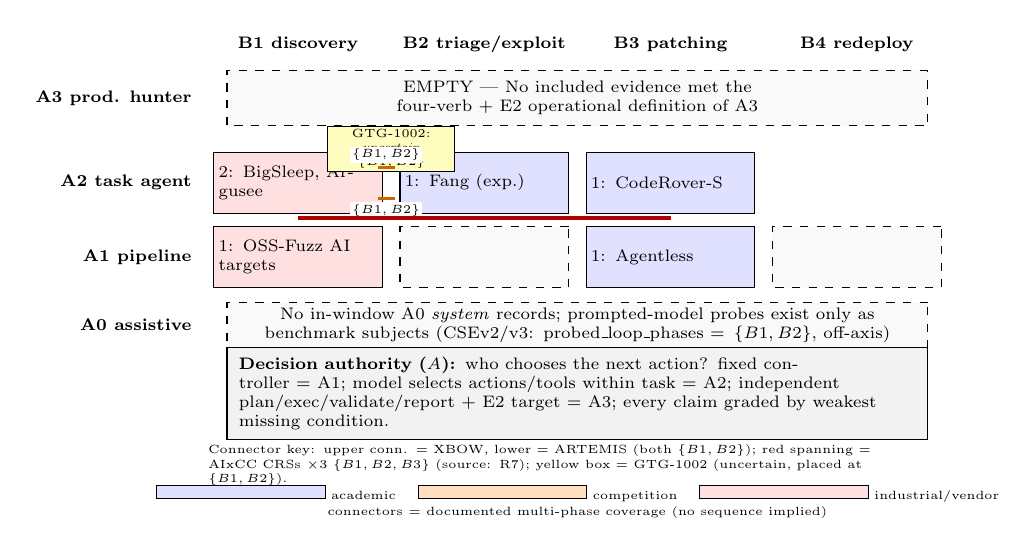
\begin{tikzpicture}[
  cell/.style={draw,align=left,font=\scriptsize,text width=2.35cm,minimum height=0.90cm,inner sep=2pt},
  acad/.style={cell,fill=blue!12}, comp/.style={cell,fill=orange!25},
  ind/.style={cell,fill=red!12}, empt/.style={cell,dashed,fill=gray!5},
  ctx/.style={draw,fill=gray!10,font=\scriptsize,align=left,text width=10.0cm,inner sep=4pt},
  lab/.style={font=\scriptsize\bfseries},
  conn/.style={-,very thick,orange!80!black},
  scale=0.86,transform shape]

% Phase headers: one shared grid.
\node[lab] at (0.0,4.30) {B1 discovery};
\node[lab] at (2.75,4.30) {B2 triage/exploit};
\node[lab] at (5.5,4.30) {B3 patching};
\node[lab] at (8.25,4.30) {B4 redeploy};

% Autonomy labels.
\node[lab,anchor=east] at (-1.45,3.50) {A3 prod. hunter};
\node[lab,anchor=east] at (-1.45,2.25) {A2 task agent};
\node[lab,anchor=east] at (-1.45,1.15) {A1 pipeline};
\node[lab,anchor=east] at (-1.45,0.15) {A0 assistive};

% A3 row.
\node[empt,minimum width=10.35cm,minimum height=0.82cm,text width=10.0cm,align=center] at (4.125,3.50)
 {\scriptsize EMPTY --- No included evidence met the four-verb $+$ E2 operational definition of A3};

% A2 row.
\node[ind]  at (0.0,2.25) {2: BigSleep, Argusee};
\node[acad] at (2.75,2.25) {1: Fang (exp.)};
\node[acad] at (5.5,2.25) {1: CodeRover-S};
% GTG-1002: narrow yellow label in B1--B2 gutter (its loop phases).
\node[font=\tiny,anchor=center,draw,fill=yellow!25,align=center,text width=1.8cm,minimum height=0.55cm,inner sep=1pt]
  at (1.375,2.75) {GTG-1002: \emph{uncertain} $\{B1,B2\}$};

% Neutral documented-coverage connectors.  The line itself stays entirely in the gutter;
% the phase-set labels sit in the whitespace immediately adjacent to that gutter.
\draw[conn] (1.175,2.48) -- (1.425,2.48);
\node[font=\tiny,anchor=south,fill=white,inner sep=1pt] at (1.30,2.53) {$\{B1,B2\}$};
\draw[conn] (1.175,2.02) -- (1.425,2.02);
\node[font=\tiny,anchor=north,fill=white,inner sep=1pt] at (1.30,1.97) {$\{B1,B2\}$};
% AIxCC is a documented B1--B3 multi-phase record; red connector spans B1--B3.
\draw[conn,red!70!black] (0.0,1.73) -- (5.5,1.73);


% A1 row.
\node[ind]  at (0.0,1.15) {1: OSS-Fuzz AI targets};
\node[empt] at (2.75,1.15) {};
\node[acad] at (5.5,1.15) {1: Agentless};
\node[empt] at (8.25,1.15) {};

% A0 note, kept inside the same B-grid.
\node[empt,minimum width=10.35cm,minimum height=0.62cm,text width=10.0cm,align=center] at (4.125,0.15)
 {\scriptsize No in-window A0 \emph{system} records; prompted-model probes exist only as benchmark
  subjects (CSEv2/v3: probed\_loop\_phases $=\{B1,B2\}$, off-axis)};

% Compact annotation band.
\node[ctx,minimum width=10.35cm] at (4.125,-0.86)
 {\textbf{Decision authority ($A$):} who chooses the next action? fixed controller $=$ A1;
  model selects actions/tools within task $=$ A2; independent plan/exec/validate/report $+$ E2 target $=$ A3;
  every claim graded by weakest missing condition.};

\node[font=\tiny,anchor=west,text width=10.35cm] at (-1.45,-1.92)
 {Connector key: upper conn. $=$ XBOW, lower $=$ ARTEMIS (both $\{B1,B2\}$); red spanning $=$ AIxCC CRSs $\times$3 $\{B1,B2,B3\}$ (source: R7); yellow box $=$ GTG-1002 (uncertain, placed at $\{B1,B2\}$).};

\node[font=\tiny,align=center] at (4.125,-2.34)
 {\tikz{\node[acad,minimum size=2mm]{};} academic \quad
  \tikz{\node[comp,minimum size=2mm]{};} competition \quad
  \tikz{\node[ind,minimum size=2mm]{};} industrial/vendor};
\node[font=\tiny,align=center] at (4.125,-2.62)
 {connectors $=$ documented multi-phase coverage (no sequence implied)};
\end{tikzpicture}
}
\caption{Autonomy $\times$ loop map over autonomy-bearing records (in-window corpus). Only
records whose unit is a system, a clearly specified experiment, or an incident documentation
receive $A$-levels (12 records, plus 2 general-SE comparators); benchmarks report \emph{probed loop phases},
datasets report \emph{task domains}, and systematization papers report \emph{documented systems}. Axis B is the
set $\{B1..B4\}$; multi-phase operation uses neutral connectors denoting documented coverage.
The A3 row is empty under the four-verb $+$ E2-environment definition; the nearest candidate
(GTG-1002) remains uncertain under the weakest-missing-condition rule.}
\label{fig:abmap}
\end{figure*}


\subsection{Migration, 2024 $\rightarrow$ June 2026}
Early in-window records are dominated by benchmarked/prompted capability evaluation, while the
system-bearing evidence shifts toward A1 pipeline automation (OSS-Fuzz's LLM stages; Agentless)
and A2 task agents --- arriving first as seeded production research (Big Sleep, November 2024),
then proliferating across independent industrial (Argusee, May 2025; XBOW, June 2025),
competition (AIxCC finals, August 2025), and production-network experimental settings (ARTEMIS).
We emphasize what this phrasing avoids: our corpus contains no in-window A0 systems, so claims
of a field-wide ``A0$\rightarrow$A1$\rightarrow$A2 migration'' would outrun the evidence; what
migrated is where humans sit (boundaries: seeds, entry points, review, reporting) and what gets
scored. The 2026 record adds consolidation --- four systematizations, an infrastructure-risk
cluster around agent tool protocols, and the first institutionalized B4 documentation.

\textbf{A3 robustness.} Under the paper's strict operational definition, no included system
qualifies as A3. This finding is robust to reasonable alternative interpretations: relaxing
the human-review rule (S1), relaxing the target-selection rule (S2), relaxing the environment
requirement (S3), and combining all relaxations (S4) each leave the A3 count at zero. The
weakest-missing-condition rule ensures that every A2 system fails at least one required condition
--- typically human-curated seeds, entry points, or pre-submission review --- preventing any
system from qualifying as A3 merely by headline claims.

% tables/autonomy-loop-matrix.tex — v4 (CP4 blocker fix): body REGENERATED from the frozen
% CP2-lock schema (14 autonomy-bearing / 2 background / 2 loop-transition-doc / 18 context).
% Root cause of prior staleness: v3 header comment updated while tabular body stayed v2.
% Source of truth: evidence/autonomy-loop-assignments.csv + corpus/included/*.yaml.
\begin{table*}[t]
\centering
\caption{Complete record-level classification (36 records). $A$ = autonomy level;
$B$ = loop-position set; T = temporal scope. Only systems, clearly specified experiments, and
incident documentation bear $A$-levels; benchmarks report probed phases ($^{p}$); datasets
report task domains; systematizations are n/a with documented systems. Per-record behavioral
evidence: \texttt{evidence/autonomy-loop-assignments.csv}.}
\label{tab:abmatrix}
\scriptsize
\setlength{\tabcolsep}{3.0pt}
\resizebox{\textwidth}{!}{%
\begin{tabular}{lllll}
\hline
Record & Year & T & $A$ & $B$-set / role \\
\hline
\multicolumn{5}{l}{\emph{(i) In-window autonomy-bearing records (14)}}\\
bigsleep2024naptime      & 2024 & in & A2        & $\{B1\}$ \\
argusee2025              & 2025 & in & A2        & $\{B1\}$ \\
fang2024one-day          & 2024 & in & A2 (exp.) & $\{B2\}$ \\
sweagent2024             & 2024 & in & A2        & $\{B3\}$ \\
autocoderoever2024       & 2024 & in & A2        & $\{B3\}$ \\
ossfuzz-aifixing2024     & 2024 & in & A2        & $\{B3\}$ \\
xbow2025                 & 2025 & in & A2        & $\{B1{+}B2\}$ \\
artemis2025comparing     & 2025 & in & A2 (exp.) & $\{B1{+}B2\}$ \\
r7-CRS-cluster recs:     &      &    &           &              \\
\quad tob-buttercup2025  & 2025 & in & A2        & $\{B1{+}B2{+}B3\}$ \\
\quad teamatlanta-sqlite2024 & 2024 & in & A2    & $\{B1{+}B2{+}B3\}$ \\
\quad teamatlanta-afc2025    & 2025 & in & A2    & $\{B1{+}B2{+}B3\}$ \\
gtg1002-2025             & 2025 & in & uncertain & $\{B1{+}B2\}$ \\
ossfuzz-levelingup2024   & 2024 & in & A1        & $\{B1\}$ \\
agentless2024            & 2024 & in & A1        & $\{B3\}$ \\
\hline
\multicolumn{5}{l}{\emph{(ii) Background anchors --- excluded from primary counts (2)}}\\
intercode2023            & 2023 & bg & A1        & $\{B2\}$ \\
csev12023                & 2023 & bg & A0        & $\{B1\}$ \\
\hline
\multicolumn{5}{l}{\emph{(iii) Loop-transition documentation --- B4 tied to systems (2)}}\\
openssfretro2026         & 2026 & in & (A2 CRS cluster) & documents $B3{\to}B4$ \\
bloggoogle-summer2025    & 2025 & in & (A2 BigSleep)    & documents $B1{\to}B4$ redeploy \\
\hline
\multicolumn{5}{l}{\emph{(iv) Off-axis / context records (18)}}\\
cybench2024              & 2024 & in & n/a & benchmark; probed $\{B2\}^p$; embedded A2-class scaffold \\
nyuctfbench2024          & 2024 & in & n/a & benchmark; probed $\{B2\}^p$; embedded A2-class scaffold \\
csev22024                & 2024 & in & n/a & benchmark; probed $\{B1,B2\}^p$ \\
csev32024                & 2024 & in & n/a & benchmark; probed $\{B1,B2\}^p$ \\
primevul2024             & 2024 & in & n/a & dataset; task domain $B1$ detection \\
rissebohme2024           & 2024 & in & n/a & methodological critique \\
mcpeco2025               & 2025 & in & n/a & MCP ecosystem measurement \\
mcpgov2025               & 2025 & in & n/a & MCP governance \\
mcpspec2026              & 2026 & in & n/a & MCP spec analysis \\
mcppoison2026            & 2026 & in & n/a & MCP tool poisoning \\
nvdcve20256965           & 2025 & in & n/a & registry record (CVE-2025-6965) \\
zhang2024when (R1)       & 2024 & in & n/a & survey (SLR) \\
r2slr2024remediation(R2) & 2024 & in & n/a & survey (SLR) \\
sheng2025csur (R4)       & 2025 & in & n/a & survey (paywalled; metadata) \\
r5usenix26agentic (R5)   & 2026 & in & n/a & survey (agentic-AI security) \\
tosemslr2026 (R6)        & 2026 & in & n/a & survey (263 studies; repo open) \\
r7sokaixcc2026 (R7)      & 2026 & in & n/a & survey(systematization); documents Atlantis, Buttercup,\\
                         &      &    &     & Theori-SRS, RoboDuck, FuzzingBrain, Lacrosse, Shellphish \\
r3survey2026pentest (R3) & 2026 & OUT& n/a & survey comparator (out-of-window) \\
\hline
\multicolumn{5}{l}{\scriptsize Totals: 14 autonomy-bearing ($A1{\times}2$, $A2{\times}11$, uncertain${\times}1$, $A3{=}0$)
$+$ 2 background $+$ 2 loop-transition $+$ 18 context $=$ 36 records.}\\
\end{tabular}
}
\end{table*}


% sections/05-discovery.tex — organized by autonomy level; evidence-grounded per corpus.
% Provenance: all cited values verified in references/txt/* extracts or local PDFs (CP1-final).
\section{Discovery: From Capability Probes to Production-Oriented Agents}
\label{sec:discovery}

Reading the in-window corpus through the decision-authority test yields a discovery landscape
that separates cleanly into pipeline automation (A1) and task-level agents (A2), with no A0
\emph{system} records: prompted-model capability probes persist only as benchmark subjects
(Sec.~\ref{sec:framework}), not as operational discoverers.

\subsection{A1: Pipeline-Orchestrated Discovery at Ecosystem Scale}
The most extensive automated discovery effort in our corpus is Google's AI-augmented
OSS-Fuzz program. Its LLM executes the first four steps of the developer fuzzing workflow ---
drafting fuzz targets, repairing compilation and runtime faults, running campaigns, and
triaging crashes into driver-vs-project attributions --- while step five (fixing) was
explicitly future work at announcement time and an agent-based architecture was listed as a
roadmap item, anchoring its A1 classification~\cite{ossfuzzlvlup2024}. The reported yield is
material: 26 new vulnerabilities across OSS-Fuzz projects, including CVE-2024-9143 in OpenSSL,
assessed by Google as likely present for two decades and ``wouldn't have been discoverable with
existing fuzz targets written by humans''~\cite{ossfuzzlvlup2024}. Two features matter for our
framework. First, the workflow controller, not the model, fixes the stage sequence --- the
defining A1 property. Second, triage automation remains pre-human-review: the authors state the
goal of reaching confidence ``not requiring human review,'' implying review persisted at
announcement time~\cite{ossfuzzlvlup2024}.

\subsection{A2: Seeded Variant Analysis in Production Code}
Project Zero's Big Sleep provides one of the earliest documented production-oriented A2 discoveries in our corpus: an
exploitable stack buffer underflow in SQLite's \texttt{seriesBestIndex}, triggered through the
\texttt{generate\_series} virtual table under a ROWID constraint, found by variant analysis over
a human-curated pool of recent commits using Gemini~1.5~Pro~\cite{bigsleep2024naptime}. Three
qualifiers discipline any capability claim. The seed pool was human-selected; the run's target
was inspired by an AIxCC finding (Sec.~\ref{sec:coevolution}); and the authors themselves note
the result is experimental and that ``a target-specific fuzzer would be at least as effective''
in general~\cite{bigsleep2024naptime}. The built-in baseline is instructive: AFL failed to
rediscover the bug after 150 CPU-hours even with a corpus pre-seeded with the required keywords,
and the OSS-Fuzz harness lacked the \texttt{generate\_series} extension entirely
--- the comparison points to harness and environment coverage as an important limiting factor; the 150 CPU-hour result does not isolate compute from harness design.
No CVE was assigned: the bug was fixed pre-release~\cite{bigsleep2024naptime}.

\subsection{A2: Entry-Point-Assisted Auditing}
DARKNAVY's Argusee distributes auditing across Manager, Auditor, and Checker agents backed by an
LSP-based code reader, and reports the discovery and analysis of CVE-2025-37891 --- an arbitrary
kernel heap overflow in the Linux USB MIDI2-to-UMP conversion path --- alongside fifteen further
vendor-reported flaws in projects such as GPAC and GIFLIB~\cite{darknavyargusee2025}. Its own
text, however, fixes the autonomy boundary: Argusee ``is not intended to completely replace
manual auditing or to discover vulnerabilities from scratch,'' operating from
\emph{human-supplied entry points}; exploitation of CVE-2025-37891 to root on Arch Linux was
performed by the human team, and Reproducer/Exploit agents are listed as future
work~\cite{darknavyargusee2025}. Argusee also reports perfect scores on CyberSecEval~2
buffer-overflow cases --- a saturation datum we return to in Sec.~\ref{sec:validity}.

\subsection{A2: Black-Box Platform Operation}
XBOW operated as a commercial submission engine across public and private HackerOne programs:
an LLM-assisted targeting layer parsed program policies, scored assets, and deduplicated
infrastructure, while internal ``validators'' re-verified findings before
submission~\cite{xbowtop12025}. The vendor reports ${\sim}1{,}060$ submissions of which 130
were resolved and 303 triaged, with 208 duplicates and 209 informative outcomes --- roughly 39
percent of submissions falling into duplicate/informative categories rather than new/resolved
findings, a metric-definition problem for leaderboard-style counting rather than simple noise
--- including a previously unknown Palo Alto GlobalProtect VPN issue affecting 2{,}000+ hosts,
for which no CVE identifier is given~\cite{xbowtop12025}. The decisive classifier for our
taxonomy is the platform rule: ``our security team reviewed them pre-submission to comply with
HackerOne's policy on automated tools''~\cite{xbowtop12025} --- independent reporting fails,
so XBOW is A2 regardless of marketing language.

\subsection{A2 Under Experiment: Production Networks}
The ARTEMIS study places six agent instances against ten professionals on the same
corporate-style network (${\sim}8{,}000$ hosts, 12 subnets), scoring the first ten hours of
sixteen-hour runs~\cite{artemis2025comparing}. We use it as environment-class E2 evidence that
agents can operate on realistic infrastructure; press-derived superiority percentages are
excluded from this paper because they do not appear in the primary text.

\subsection{Cross-Cutting Comparison}
Table~\ref{tab:disccompare} consolidates the discovery records. Reading down the autonomy
column, the pattern consistent with I1 is cross-sectional rather than longitudinal: every record retains an
identified human locus (seed curation, entry points, mandatory review, target selection), and what
we observe is that human involvement increasingly appears at the boundaries of the autonomous
workflow --- seed selection, target selection, entry-point specification, final reporting --- rather
than on each individual tool action, while evaluation, funding, and discourse increasingly score
systems by their degree of autonomous operation.

\begin{table}[t]
\centering\scriptsize
\caption{Discovery-side comparison across autonomy levels. E-class per protocol v4;
validity flags use the V1--V5 taxonomy of Sec.~\ref{sec:validity}. All production statistics are
vendor-reported unless noted.}
\label{tab:disccompare}
\resizebox{\columnwidth}{!}{%
\begin{tabular}{p{1.55cm}llp{1.5cm}p{1.6cm}p{1.7cm}}
\hline
Record & $A$/E & Human locus & Metric & Baseline & Validity risks\\
\hline
OSS-Fuzz AI \cite{ossfuzzlvlup2024} & A1/E2 & report review & 26 vulns; CVE-2024-9143 &
 prior harnesses & V5 triage counts\\
Big Sleep \cite{bigsleep2024naptime} & A2/E2 & curated seeds & n=1 find + repro &
 AFL 150 CPU-h fail & V1 model preknowledge\\
Argusee \cite{darknavyargusee2025} & A2/E2 & entry points & CVE-2025-37891; 15 claims &
 CSEv2 100\% (sat.) & self-adjudication\\
XBOW \cite{xbowtop12025} & A2/E2 & mandated review & funnel stats; rank & leaderboard &
 unaudited dashboard\\
ARTEMIS \cite{artemis2025comparing} & A2/E2 & comparison arm & first-10h score & professionals &
 single environment\\
\hline
\end{tabular}}
\end{table}

% sections/06-exploitation.tex — AIxCC treated as competition + system-design case (spec §6).
\section{Exploitation and Validation: The AIxCC Case Study}
\label{sec:aixcc}

The Defense Advanced Research Projects Agency's Artificial Intelligence Cyber Challenge
(AIxCC) is the only included setting in our corpus where discovery, proof-of-vulnerability
generation, and patching were integrated, scored, and operated without human intervention --- and it is best
analyzed not as a benchmark but as a deliberately constructed offense$\leftrightarrow$defense
instrument whose rules, incentives, and aftermath document how the field's unit of progress was
administratively redefined (I1). Beyond competition settings, recent benchmarks such as
CVE-Bench~\cite{cvebench2025} evaluate LLM agents on real-world web application vulnerabilities,
reporting that state-of-the-art agent frameworks exploit up to 13\% of critical-severity CVEs in
sandboxed environments. Multi-agent red-teaming frameworks like Co-RedTeam~\cite{coredteam2026}
demonstrate that orchestrated discovery and exploitation stages, grounded in execution feedback
and long-term memory, achieve over 60\% success rates on exploitation tasks across multiple
security benchmarks. CyberGym~\cite{cybergym2025} further scales evaluation to real-world
vulnerabilities at industrial scale, providing evidence on the computational costs and failure
modes of agentic exploitation.

\subsection{Design and Incentives}
Announced in 2023 with ARPA-H participation and support from Anthropic, Google, Microsoft, and
OpenAI, the challenge funneled 42 accepted semifinal teams down to seven finalists, each
receiving \$2M to harden a Cyber Reasoning System (CRS) for a final round ``set up to mimic a
real world CI/CD pipeline''~\cite{openssfaixcc2026}. Scoring rewarded finding vulnerabilities,
proving them via PoVs, and applying correct patches, with speed and accuracy modifiers;
``human interaction was strictly prohibited'' during scored operation~\cite{tobbuttercup2025}.
Two incentive details matter for interpretation. Patching was worth three times discovery
(6 vs.\ 2 points), making B3 capability the rational investment~\cite{taasc2024}; and accuracy
modifiers penalized incorrect patches quadratically --- Team Atlanta reports its PoV-validated
91.27\% patch accuracy yielding a modifier of $1-(1-0.9127)^4=0.9999$ against Theori's
PoV-free $44.4\%$ yielding $0.9044$~\cite{taafc2025}. The scoring mathematics thus priced
patch-quality adjudication directly into strategy.

\subsection{What the Final Round Measured}
Participant and systematization primaries agree on the scored structure: 48 challenge projects
across 23 open-source repositories in the final round~\cite{tobbuttercup2025}, operated over
what the systematization records as ``143 hours of fully autonomous operation'' by CRSs from
all seven finalist teams~\cite{r7sokaixcc2026}. Crucially, the CRSs also surfaced real,
non-synthetic vulnerabilities --- Team Atlanta reports six C/C++ and twelve Java bugs found
collectively during the final, including a SQLite zero-day first seen at
semifinals~\cite{taafc2025} --- and Trail of Bits demonstrated a PoV for a vulnerability that
had \emph{not} been inserted into any challenge~\cite{tobbuttercup2025}. Real-bug discovery did
not score --- Team Atlanta footnotes that their autonomous find-and-patch of a real SQLite bug
during semifinals earned nothing competitively~\cite{taasc2024} --- yet it is precisely this
unscored spillover that connects the competition to the production ecosystem. DARPA's official
closeout reports the remaining aggregates: competitors' systems discovered 54 of 63 synthetic
vulnerabilities (86\%) and patched 43 (68\%), alongside 11 patches for the real
vulnerabilities~\cite{darparesults2025}; DARPA's scoring guide separately confirms both the
three-to-one patching incentive and the \$8.5M final prize pool~\cite{darpascoring2025}. The
closeout also carries an editor's note correcting its own earlier count of 70 synthetic
vulnerabilities to 63 --- an instance of administrative record instability we separate from
measurement validity throughout (Sec.~\ref{sec:validity}).

\subsection{CRS Design Space}
The finalist architectures span the design axes our framework distinguishes.
\emph{Atlantis} (Team Atlanta) ran N-version programming across orthogonal sub-CRSs (C, Java,
multilanguage, patching, SARIF), ensemble fuzzing and concolic execution alongside LLM agents,
and an explicit integration taxonomy --- LLM-augmented, LLM-opinionated, LLM-driven ---
with smaller models often outperforming larger or reasoning models for patch tasks; its
validation oracle re-runs PoVs against patched builds while acknowledging that MTE/PAC
recompilation or broad \texttt{catch(Exception)} wrappers can suppress PoVs without semantic
repair~\cite{taafc2025}. \emph{Buttercup} (Trail of Bits) took the opposite bet:
deterministic, expertise-decomposed workflows with LLMs only where classical tools fail,
using exclusively non-reasoning models --- achieving the field's best cost efficiency at
\$181 per point (versus Atlanta's \$263) on 28 vulnerabilities and 19 patches across 20 CWE
classes with ${>}90\%$ accuracy~\cite{tobbuttercup2025,r7sokaixcc2026}. \emph{Theori}
demonstrated purely static, PoV-free patching, trading accuracy for robustness to absent
proofs~\cite{taafc2025}. Team-level compute costs are independently consistent across our two
sources: totals of \$103.3K (Atlanta), \$39.6K (Trail of Bits), and \$31.8K (Theori) appear in
both the systematization analysis and the participant account~\cite{r7sokaixcc2026,tobbuttercup2025}.

\subsection{Brittleness as Environment Evidence}
The most cited lesson inside the winning team is a string-matching heuristic: Atlantis skipped
patch generation for paths containing ``fuzz,'' and organizers' ``ossfuzz'' directory prefixing
nearly disabled the system hours before the deadline --- ``here we were, building an autonomous
CRS powered by state-of-the-art AI, nearly defeated by a string matching bug''~\cite{taafc2025}.
For our validity taxonomy this is textbook V4: benchmark-specific heuristics functioned as
load-bearing components, invisible until the environment shifted.

\subsection{Architecture Lessons and the Epistemics of A3}

\label{sec:aixcc-epistemics}

The finalist designs instantiate three distinct philosophies about where intelligence belongs

in a CRS. Atlantis distributes it across N-version programming: independent sub-systems for

C, Java, multilanguage discovery, patching, and SARIF bundling, deliberately orthogonal so a

failure in one does not cascade --- with ensembling explicitly framed as the engineering

answer to LLM non-determinism (``what the ML community calls hallucination, systems engineers

call non-determinism'')~\cite{taafc2025}. Buttercup concentrates expertise in deterministic

decomposition, integrating LLMs ``only where traditional tools fall short,'' augmenting

libFuzzer and Jazzer with LLM-generated test cases behind a multi-agent patcher with

separation of concerns --- and reports that this discipline, not model scale, drove its

efficiency: \$181 per competition point using exclusively non-reasoning models, versus \$263

for the winner~\cite{tobbuttercup2025}. Theori bet on removing the runtime oracle entirely,

producing correct patches by pure static analysis at 44.4\% accuracy --- a strategy the

accuracy-modifier formula priced heavily but did not disqualify~\cite{taafc2025}.

Two quantitative facts refine any capability narrative. First, model scale inverted where it

mattered most: smaller models ``often outperformed larger foundation models and even reasoning

models'' for patch generation~\cite{taafc2025}, echoing scaffold-over-scale findings elsewhere

in our corpus. Second, validation infrastructure capped agent counts: re-verifying one nginx

patch takes ten-plus minutes, so Atlantis ran six patching agents rather than sixty ---

a reminder that B3 scaling is gated by build-and-test throughput, not tokens.

The competition also yields its cleanest end-to-end A2 datapoint. During semifinals, Atlantis

autonomously identified and patched a real SQLite FTS5 vulnerability --- an off-by-one read in

the trigram tokenizer reaching a NULL dereference --- in roughly fifteen minutes spanning

build, patch generation, iteration, and validation; the maintainer's subsequent fix

(commit e9b919d5) extended the pattern to sibling tokenizer functions and was itself revised

in a follow-up commit~\cite{taasc2024}. Discovery and repair here were performed by the system;

the exploit-to-root-privilege demonstration afterward was not.

What AIxCC can and cannot establish follows directly. It demonstrates integrated

$\{B1,B2,B3\}$ operation with execution autonomy under active prohibition of human input ---

the strongest documented autonomy evidence in our corpus. It cannot certify A3: challenges

are forked repositories carrying inserted bugs (environment class E1, not E2), real-bug

discovery went unscored, and DARPA has not released the telemetry that would let outsiders

audit either claim~\cite{tobbuttercup2025}. Post-competition triage sharpened the point rather

than resolving it: Ada Logics reproduced twenty-seven candidate real issues, while other

findings dissolved into already-fixed code, project threat-model exclusions, or known

OSS-Fuzz reports~\cite{openssfaixcc2026} --- outcome adjudication, not discovery, was the

binding difficulty.

\subsection{Interpretive Discipline}
Three boundaries govern what AIxCC evidence can support. First, E-class: competition forks with
inserted bugs are environment E1; substantial autonomy under prohibition of human interaction
still fails A3's production-environment condition. Second, outcome definitions: ``discovered''
means a scored synthetic-vulnerability PoV, ``patched'' means oracle-passing --- the oracle-gaming
taxonomy above bounds what ``correctly patched'' certifies. Third, record reliability: figures
here cite corrected primaries (DARPA closeout, participant blogs cross-checked against the
systematization), never press intermediaries. With those bounds, AIxCC demonstrates that
integrated $\{B1{+}B2{+}B3\}$ operation at A2 is achievable within one engineering generation
--- and its aftermath, examined in Sec.~\ref{sec:coevolution}, shows the loop continuing
through funded redeployment rather than ending at a scoreboard.

% sections/07-patching.tex — B3 stream + AIxCC patching lessons + blind spots (spec §7).
\section{Patching: The B3 Stream and Its Blind Spots}
\label{sec:patching}

For a title promising discovery, exploitation, \emph{and} patching, B3 is where the in-window
corpus is thinnest --- and where its structure is therefore most informative. Autonomous repair
evidence arrives through two independent channels: a general software-engineering agent lineage
repurposed for security, and the competition crucible of Sec.~\ref{sec:aixcc}.

\subsection{The Agent Lineage}
Three 2024 systems establish the design contrast that our decision-authority test formalizes.
SWE-agent demonstrates that interface design --- the agent--computer interface through which the
model issues file, search, and edit actions --- governs autonomous issue-resolution
performance~\cite{sweagent2024}. AutoCodeRover operationalizes iterative,
program-structure-aware localization and repair, letting the model decide which repository
context to request next~\cite{autocoderoever2024}. Agentless deliberately inverts the design
point: a fixed localize$\rightarrow$repair$\rightarrow$validate pipeline with no dynamic action
selection matches or beats agentic baselines at lower cost~\cite{agentless2024}. The security
specialization of this lineage, CodeRover-S, repurposes AutoCodeRover against OSS-Fuzz
vulnerabilities and states the distinction explicitly: ``having autonomy in the LLM agent is
useful for successful security patching, as opposed to approaches like Agentless where the
control flow is fixed''~\cite{ossfuzzfix2024}. Its mechanism satisfies our test at the action
level --- the model invokes AST search, file navigation, compilation, and test-execution tools,
gathering failure information before committing patches~\cite{ossfuzzfix2024}. Reported efficacy
on real OSS-Fuzz vulnerabilities remains far from saturation (52.4\% on a curated set under the
paper's conditions), and validation is sanitizer/test-based rather than exploit-aware ---
precisely the gap AIxCC's oracle-gaming taxonomy names. CVE-Genie reproduces approximately 51\%
of CVEs published in 2024--2025 with verifiable exploits at an average cost of \$2.77 per
CVE~\cite{cvegenie2025}, demonstrating the feasibility of automated vulnerability reproduction
at scale. Recent surveys systematize the broader landscape of LLM-based automated program
repair~\cite{llmaprsurvey2026}, identifying four paradigms: fine-tuning, prompting, procedural,
and agentic workflows. On the security-specific repair side, tree-of-thought prompting with
execution-log feedback achieves substantially higher patch correctness than direct generation on
real-world vulnerability datasets~\cite{logsinpatchesout2025}, suggesting that structured
reasoning over repair candidates --- rather than single-shot generation --- is an important
design choice for B3 systems. LLM4CVE~\cite{llm4cve2025} extends this line with an iterative
pipeline that combines traditional bug repair methods with LLM techniques, demonstrating
automated vulnerability repair in critical system software with minimal human input.
RepoAudit~\cite{repoaudit2025} operationalizes autonomous repository-level code auditing,
demonstrating that LLM-agents can systematically analyze large codebases for security
vulnerabilities. These systems, together with the agent lineage above, establish that
B3 capability now spans from pipeline-orchestrated repair (Agentless) through iterative
agentic workflows (AutoCodeRover, CodeRover-S) to fully autonomous auditing (RepoAudit)
--- yet exploit-aware validation remains the bottleneck across all approaches.

\subsection{What the Competition Taught About Repair Quality}
AIxCC provides the corpus's largest competition-based stress test of automated patching. Its lessons
map directly onto validity axis V5: PoV re-execution establishes behavior only for the tested proof --- it does not certify semantic correctness;
recompilation with MTE/PAC or broad exception wrapping can pass without repairing root causes,
so teams built additional oracles (optional \texttt{test.sh}) and accuracy modifiers became the
binding score component~\cite{taafc2025}. Patch correctness is itself iterative and review-dependent:
the SQLite maintainer's own fix for the FTS5 bug initially added redundant checks to sibling
tokenizer functions and required revision in a follow-up commit~\cite{taasc2024}. Ensemble
patching emerged as the dominant mitigation for LLM non-determinism --- Atlantis capped its
patching agents at six not by principle but because validating one nginx patch takes ten-plus
minutes~\cite{taafc2025}, an infrastructure constraint on B3 scaling that no benchmark measures.

\subsection{Blind Spots}
Four gaps bound current evidence. (i)~\emph{Exploit-aware validation}: outside competition
scoring, no corpus system validates that a patch removes exploitability rather than a symptom;
the PoV-as-oracle literature begins and largely ends with AIxCC artifacts~\cite{patcheval2025}.
(ii)~\emph{Regression and redeployment}: B4 exists in our corpus solely as foundation-documented
ecosystem transition --- OpenSSF SIG hosting, \$200K-per-team integration funding, Team Atlanta's
\$2M prize recycling into continuous hunting~\cite{openssfaixcc2026,tobbuttercup2025,taafc2025}
--- never as an academic evaluation target with regression metrics. (iii)~\emph{Attacker
adaptation}: no included work studies adversaries reacting to deployed auto-patchers; the
offensive side of B3 is absent. (iv)~\emph{Interaction with discovery}: patching and discovery
are evaluated as separate competencies everywhere except inside CRS pipelines; whether autonomous
discovery changes patch demand or maintainer workload at ecosystem scale is unmeasured (DARPA has
not yet released the telemetry that would permit it~\cite{tobbuttercup2025}). These gaps seed
the roadmap experiments of Sec.~\ref{sec:roadmap}.

% sections/08-coevolution.tex — graded coupling edges; headline per protocol v4 claim ledger.
\section{The Co-Evolution Loop: Graded Evidence}
\label{sec:coevolution}

Our second insight concerns coupling between offense and defense. We grade every candidate edge
on a three-level scale --- \emph{documented response} (an explicit, sourced statement or
traceable institutional flow), \emph{plausible coupling} (mechanism-reasonable temporal
adjacency), and \emph{temporal association} (chronology alone) --- and claim only what the
grades support: multiple documented edges exist; field-wide causal co-evolution does not follow
from them.

\subsection{Documented Response Edges}
\textbf{(D1) Competition $\rightarrow$ industrial research program.} Project Zero's Big Sleep
post opens its target rationale by citing the challenge directly: ``Earlier this year at the
DARPA AIxCC event, Team Atlanta discovered a null-pointer dereference in SQLite, which inspired
us to use it for our testing''~\cite{bigsleep2024naptime}. This is the corpus's cleanest causal
edge: named source, stated mechanism, dated.
\textbf{(D2) Maintainer-side variant response.} After Atlantis reported the FTS5 trigram
off-by-one, the SQLite maintainer patched not only the reported function but sibling tokenizer
code paths sharing the pattern, then revised his own patch in a follow-up commit after noting
redundancy~\cite{taasc2024} --- human variant analysis triggered by an AI finding.
\textbf{(D3) Institutional/funding flows.} The loop acquired governance: DARPA and ARPA-H
committed \$200K per team to integrate CRSs into critical software~\cite{tobbuttercup2025};
Team Atlanta recycled half its \$4M prize (\$2M) into continuous autonomous hunting at Georgia
Tech's SSLab with OpenAI contributing API credits~\cite{taafc2025}; OpenSSF chartered a Cyber
Reasoning Systems SIG and hosts OSS-CRS and FuzzingBrain, whose post-competition operation is
reported at 62 vulnerabilities across 26 projects (43 maintainer-confirmed, 36 patched upstream)
for FuzzingBrain and 25 vulnerabilities across 16 projects for OSS-CRS~\cite{openssfaixcc2026}.
These are foundation-relayed, team-reported figures; the funding and governance mechanisms provide evidence that competition-derived capabilities persisted beyond the scored event.
\textbf{(D4) Threat-seeded defensive disclosure.} Google's CVE-2025-6965 disclosure couples its
Threat Intelligence unit to Big Sleep: the flaw was ``known only to threat actors,'' and the
company asserts an imminent exploit was cut off --- ``we believe this is the first time an AI
agent has been used to directly foil efforts to exploit a vulnerability in the
wild''~\cite{bloggoogle2025,nvd6965}. The threat-intelligence premise is unverifiable and the
foiling counterfactual; we cite it as documented defensive process, not verified attack
prevention.

\subsection{Plausible Coupling}
\textbf{(P1)} Attacker-side adoption of agentic operation within roughly twelve months of
defender agentic publicity: Anthropic reports GTG-1002 used Claude Code for 80--90\% of an
espionage campaign's execution --- ``the AI autonomously discovered vulnerabilities in targets
selected by human operators''~\cite{anthropicgtgreport2025,anthropicgtg2025}. Directionality is
unverifiable without adversary telemetry; shared capability tide remains a live alternative.

\subsection{Temporal Association Only}
Benchmark releases trailing industrial demos, press arms-race narratives, and leaderboard
movements populate this tier; per our claim ledger they carry no inferential weight here.

\subsection{Falsification Test and Record Reliability}
The shared-cause objection --- frontier-model releases independently advancing both sides ---
survives globally: it is defeated only for edges D1--D2, where stated mechanisms precede any
model-release timing argument. We therefore do not generalize from the AIxCC--Google hub to the
field. Record reliability itself becomes evidence, once accounting scopes are labeled precisely:
\$29.5M denotes the cumulative program prize commitment announced in 2024, \$8.5M denotes the
final competition pool per DARPA's scoring guide~\cite{darpascoring2025}, and OpenSSF reports
\$30.5M ultimately distributed across both rounds~\cite{openssfaixcc2026} --- distinct
boundaries, not competing totals for one quantity. Separately, DARPA's own closeout corrects
its earlier synthetic-vulnerability count from 70 to 63~\cite{darparesults2025}: an
administrative record correction showing that even authoritative primary sources require
version- and date-aware verification.



% figures/timeline-f3.tex — F3: capability timeline 2023–2026 (layout-aligned revision)
% Every date cross-checked against Appendix C / claim-verification.csv.
\begin{figure*}[t]
\centering
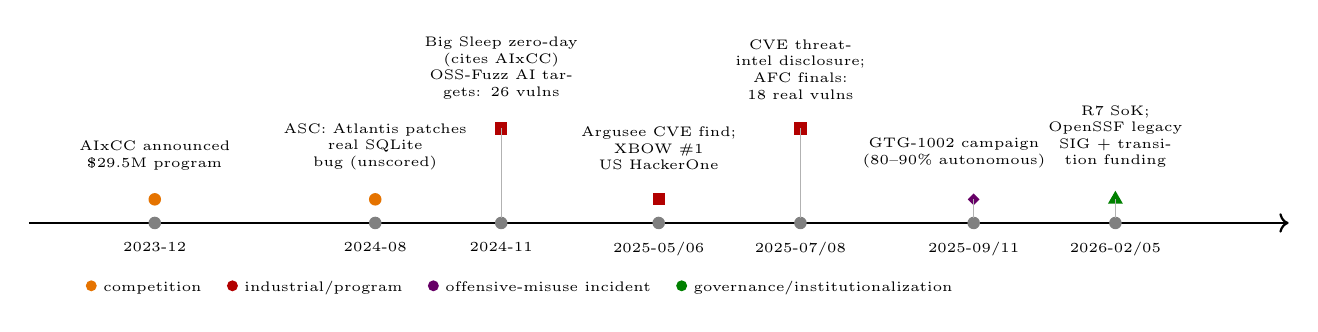
\begin{tikzpicture}[
  ev/.style={font=\tiny,align=center,text width=2.55cm},
  dot/.style={circle,fill,inner sep=1.6pt},
  comp/.style={dot,orange!90!black}, ind/.style={dot,red!70!black,shape=rectangle,inner sep=2.2pt},
  mis/.style={dot,violet!80!black,diamond,inner sep=1.1pt}, gov/.style={dot,green!50!black,shape=regular polygon,regular polygon sides=3,inner sep=1.1pt},
  scale=1.0,transform shape]
\draw[->,thick] (-0.4,0) -- (15.6,0);
\foreach \x/\lab in {1.2/{2023-12},4.0/{2024-08},5.6/{2024-11},7.6/{2025-05/06},
                     9.4/{2025-07/08},11.6/{2025-09/11},13.4/{2026-02/05}} {
  \node[ev,below,text width=1.8cm] at (\x,-0.12) {\lab};
  \node[dot,gray] at (\x,0) {};
}
% Event labels are deliberately staggered so neighboring annotations never collide.
\node[ev,anchor=south] at (1.2,0.55) {AIxCC announced\\ \$29.5M program};
\node[comp] at (1.2,0.30) {};
\node[ev,anchor=south] at (4.0,0.55) {ASC: Atlantis patches\\ real SQLite bug (unscored)};
\node[comp] at (4.0,0.30) {};
\node[ev,anchor=south] at (5.6,1.45) {Big Sleep zero-day (cites AIxCC)\\ OSS-Fuzz AI targets: 26 vulns};
\node[ind] at (5.6,1.20) {}; \draw[gray!60] (5.6,1.20)--(5.6,0.06);
\node[ev,anchor=south] at (7.6,0.55) {Argusee CVE find;\\ XBOW \#1 US HackerOne};
\node[ind] at (7.6,0.30) {};
\node[ev,anchor=south] at (9.4,1.45) {CVE threat-intel disclosure;\\ AFC finals: 18 real vulns};
\node[ind] at (9.4,1.20) {}; \draw[gray!60] (9.4,1.20)--(9.4,0.06);
\node[ev,anchor=south] at (11.35,0.58) {GTG-1002 campaign\\ (80--90\% autonomous)};
\node[mis] at (11.6,0.30) {}; \draw[gray!60] (11.6,0.30)--(11.6,0.06);
\node[ev,anchor=south,text width=2.4cm] at (13.40,0.58) {R7 SoK; OpenSSF legacy\\ SIG + transition funding};
\node[gov] at (13.4,0.30) {}; \draw[gray!60] (13.4,0.30)--(13.4,0.06);
% legend
\node[font=\tiny,anchor=west] at (0.2,-0.82)
 {\tikz{\node[comp,inner sep=1.4pt,circle,fill=orange!90!black]{};} competition \quad
  \tikz{\node[ind,inner sep=1.4pt,circle,fill=red!70!black]{};} industrial/program \quad
  \tikz{\node[mis,inner sep=1.4pt,circle,fill=violet!80!black]{};} offensive-misuse incident \quad
  \tikz{\node[gov,inner sep=1.4pt,circle,fill=green!50!black]{};} governance/institutionalization};
\end{tikzpicture}
\caption{Capability-and-coupling timeline for the graded edges of Sec.~VIII. Colors separate
evidence classes; every event carries a primary source in Appendix~\ref{app:timeline}. The
sequence visualizes I2's documented edges --- most notably the AIxCC$\rightarrow$Big Sleep
inspiration link --- without implying field-wide causal closure.}
\label{fig:f3timeline}
\end{figure*}

\subsection{Temporal Association Only}
Benchmark releases trailing industrial demos, press arms-race narratives, and leaderboard
movements populate this tier; per our claim ledger they carry no inferential weight here.

\subsection{Falsification Test and Record Reliability}
The shared-cause objection --- frontier-model releases independently advancing both sides ---
survives globally: it is defeated only for edges D1--D2, where stated mechanisms precede any
model-release timing argument. We therefore do not generalize from the AIxCC--Google hub to the
field. Record reliability itself becomes evidence, once accounting scopes are labeled precisely:
\$29.5M denotes the cumulative program prize commitment announced in 2024, \$8.5M denotes the
final competition pool per DARPA's scoring guide~\cite{darpascoring2025}, and OpenSSF reports
\$30.5M ultimately distributed across both rounds~\cite{openssfaixcc2026} --- distinct
boundaries, not competing totals for one quantity. Separately, DARPA's own closeout corrects
its earlier synthetic-vulnerability count from 70 to 63~\cite{darparesults2025}: an
administrative record correction showing that even authoritative primary sources require
version- and date-aware verification.

\subsection{Institutional Response}

Between one-off response and field-level causation sits a grade our corpus documents richly:

institutionalization. Three funding and governance flows carry competition-derived capability

past the scoreboard. DARPA and ARPA-H committed \$200K per finalist team to integrate CRSs

into critical software~\cite{tobbuttercup2025}. Team Atlanta recycled half of its \$4M prize

into continuous autonomous hunting of OSS-Fuzz projects at Georgia Tech's SSLab, with OpenAI

contributing API credits~\cite{taafc2025}. And OpenSSF chartered a Cyber Reasoning Systems

Special Interest Group that now hosts OSS-CRS and FuzzingBrain, relaying post-competition

yields --- sixty-two vulnerabilities across twenty-six projects for FuzzingBrain

(forty-three maintainer-confirmed, thirty-six patched upstream), twenty-five vulnerabilities

across sixteen projects for OSS-CRS, and twelve kernel-related plus ten user-space zero-day

findings for 42-b3yond-6ug~\cite{openssfaixcc2026}. These counts remain team-relayed; the

institutions, budgets, and standing governance are independently observable. Google's parallel

commitment --- deploying Big Sleep against widely used open-source projects~\cite{bloggoogle2025}

--- extends the same pattern from competition lineage to industrial program.

On the speculative side of the ledger sits attacker-side adoption. The strongest candidate is

GTG-1002: a framework wrapping Claude Code with MCP tool access, jailbroken through task

decomposition and fabricated defensive-employment framing, executing reconnaissance,

exploit drafting, credential harvesting, and exfiltration with humans selecting targets and

intervening at four to six checkpoints~\cite{anthropicgtg2025,anthropicgtgreport2025}. Its

grade stays \emph{plausible coupling}: no adversary-side telemetry exists to date whether

defender publications caused, accelerated, or merely coincided with the technique transfer.

A concrete falsifier structures future work: if adoption-lag measurement finds agentic

offensive techniques appearing no earlier after major defender disclosures than baseline

diffusion rates would predict, response-coupling loses its offensive half and I2 narrows to

defender-internal loops.

\subsection{Summary}
The loop is real where it is documented: a competition generated tooling whose inspiration
seeded an industrial program (D1), whose findings triggered maintainer responses (D2), whose
participants now operate continuously under foundation governance (D3), and whose defender
capability claims now interleave with threat-intelligence-driven disclosure (D4). What the
record cannot yet support is the stronger vernacular claim of an ongoing arms race; that
requires adversary-side measurement this corpus lacks (Sec.~\ref{sec:roadmap}).

% sections/09-validity.tex — §9: validity as first-class measurement (spec §6 protocol).
\section{Evaluation Validity}
\label{sec:validity}

Our third insight treats validity as a measurable property of evaluations, not a limitations
paragraph. We organize the evidence as a progression --- information leakage, then dataset-level
invalidity, then oracle manipulation --- because each tier changes what a reported number can
mean.

\subsection{V2/V3: Information Leakage, Measured by Intervention}
The cleanest datum in our corpus is controlled. Fang et al.\ measure GPT-4-based agents on 15
real one-day vulnerabilities under two information conditions: with the CVE description
supplied, the agent autonomously exploited 87\%; without it, success fell to 7\%, while every
baseline (GPT-3.5, eight open-source models, ZAP, Metasploit) scored zero in both
conditions~\cite{fang2024agents}. The twelve-fold swing is produced by a single
supplied-knowledge variable --- the CVE text functions as a partial answer key --- so any
capability claim inherits its information condition. We therefore report such results only with
their conditions attached, and the same discipline applies to temporal leakage: every
vulnerability in that benchmark was publicly disclosed before model training cutoffs.

\subsection{V1/V5: Dataset-Level Invalidity, Measured by Reconstruction}
PrimeVul demonstrates that the detection literature's benchmark layer was structurally
unsound: label noise, near-duplicate pairs across splits, and pre-split public exposure
inflated reported performance to the point where paired, chronologically split evaluation
collapses strong-model accuracy toward chance~\cite{primevul2024}. Risse and B\"ohme reach a
compatible verdict from measurement theory, arguing that popular vulnerability datasets score
models on the wrong exam~\cite{rissebohme2024}. The corpus also contains a live saturation
illustration: Argusee reports 100\% on CyberSecEval~2 buffer-overflow cases while its own
documentation requires human-supplied entry points~\cite{darknavyargusee2025} --- ceiling
scores coexisting with bounded autonomy. Agentic CTF suites inherit a further V1 exposure:
their tasks derive from publicly written-up competitions, and no included work quantifies the
inflation this induces; we return to it as roadmap experiment E2.

\subsection{V4/V5: Oracle Manipulation and Environment Brittleness, Documented Operationally}
AIxCC supplied operational evidence on outcome definitions. PoV re-execution establishes
behavior only for the tested proof; teams documented mitigation-gaming patches --- recompiling
with MTE/PAC or wrapping entry points in broad \texttt{catch} blocks --- that pass PoVs without
semantic repair, prompting optional functional tests as secondary oracles and an accuracy
modifier that made patch correctness the binding score term~\cite{taafc2025}. Environment
leakage is exemplified by the winning CRS nearly disabling itself when organizers prefixed
challenge directories with ``ossfuzz,'' breaking a ``fuzz''-substring heuristic --- load-bearing
benchmark-specific logic invisible until the environment shifted~\cite{taafc2025}. On the
production side, leaderboard-style counting conflates heterogeneous outcomes: of XBOW's
${\sim}1{,}060$ submissions, roughly 39\% resolved into duplicate or informative categories
rather than new/resolved findings --- categories that reflect discovery overlap and program
policy as much as agent error, making rank non-decomposable without category-aware
accounting~\cite{xbowtop12025}.

\subsection{Administrative Record Correction: A Separate Category}
DARPA's closeout corrects its own synthetic-vulnerability count from 70 to 63 with an editor's
note~\cite{darparesults2025}, and prize accounting requires three scoped figures rather than
one (\$29.5M cumulative commitment, \$8.5M final pool, \$30.5M
distributed~\cite{darpascoring2025,openssfaixcc2026}). These are administrative record
corrections, not measurement-validity failures, but they carry a methodological moral we adopt
as policy: even authoritative primary sources require version- and date-aware verification,
and press intermediaries inherit whatever instability the primary contains.

\subsection{A Contamination-Control Protocol}
As a concrete deliverable, we specify the minimal protocol any agentic capability evaluation
should publish: (i)~\emph{temporal firewall} --- freeze the task set at date $T$, evaluate only
models whose training cutoffs precede $T-\Delta$ for disclosed $\Delta$, and release the task
set only after evaluation; (ii)~\emph{provenance screening} --- machine-check every task against
public write-up corpora and NVD text up to $T$, reporting overlap rates rather than asserting
cleanliness; (iii)~\emph{information-condition disclosure} --- state exactly which artifacts
(descriptions, patches, stack traces, credentials) are supplied to the agent, Fang-style;
(iv)~\emph{category-aware outcomes} --- report validated/exploitable/duplicate/informative as
separate counts with adjudication rules fixed before running; and (v)~\emph{adjudication
audit} --- a second scorer re-labels a random 10\% sample with agreement statistics. No
included evaluation satisfies all five today; E3 (Sec.~\ref{sec:roadmap}) operationalizes the
gap.

\subsection{The Measured Core, Quantified}

Three numbers anchor the progression above; each survives re-examination better than the

headline claims it corrects. Fang et al.'s intervention separates information supply from

capability: Pass@5 of 86.7\% and an overall exploitation rate of 40\% for GPT-4 under

description-supplied conditions collapse to 7\% overall without descriptions, while GPT-3.5,

eight open-source models, ZAP, and Metasploit score zero throughout~\cite{fang2024agents} ---

the condition, not the model, carries the result. PrimeVul's reconstruction moves a

state-of-the-art 7B detector from 68.26\% F1 on BigVul to 3.09\% on its paired,

chronologically split evaluation, with GPT-3.5- and GPT-4-class prompting ``akin to random

guessing'' under the most stringent settings~\cite{primevul2024} --- dataset construction, not

model capacity, had been the binding constraint on prior comparisons. And XBOW's funnel makes

outcome-definition noise concrete at production scale: of ${\sim}1{,}060$ submissions, 208

duplicates and 209 informative reports --- roughly 39\% --- resolve into neither new nor fixed

findings, so leaderboard position aggregates discovery quality with program-policy artifacts

unless category-aware accounting is applied~\cite{xbowtop12025}. Each datum predates or

operates independently of the others; their convergence on the same methodological conclusion

is why we treat validity as measured rather than alleged.

\subsection{What Survives}
Validity constraints do not render the corpus uninterpretable. Condition-controlled results
survive (the 7\% no-description condition), third-party adjudication survives (Ada Logics'
reproduction of 27 AIxCC-derived issues~\cite{openssfaixcc2026}), and platform triage provides
weak external checks on vendor claims. What does not survive is unqualified headline numbers ---
which are precisely the ones that travel furthest.

% sections/10-threats.tex — §10 threats to validity of the SoK itself.
\section{Threats to Validity}
\label{sec:threats}

\textbf{Publication and visibility bias.} Our industrial stream consists of organizations that
\emph{publish}: Google, Anthropic, XBOW, DARKNAVY, OpenSSF. Systems that operate silently ---
commercial pentesting vendors, state programs, internal red teams --- are structurally
invisible, so our A3-empty finding is a statement about documented evidence, not about private
capability. Proprietary disclosure is incomplete even where marketing is not.

\textbf{Survivor and selection bias.} Vendors report successes; failed autonomous deployments
rarely generate blog posts. XBOW's funnel (208 duplicates, 209 informative) is published only
because its denominator was large enough to survive; smaller negative results have no venue.

\textbf{Source-quality asymmetry.} Academic records carry methods sections; vendor records
carry dashboard screenshots. We mitigate with quote-level extraction, cross-source
corroboration where possible (AIxCC cost tables agree across participant and systematization
primaries), and explicit CLAIMED labels --- but asymmetry remains, and one vendor-reported
incident (GTG-1002) materially shapes the autonomy frontier of our corpus.

\textbf{Rapid model churn.} Capabilities tracked here span Gemini~1.5 Pro through mid-2026
models; any conclusion phrased about ``LLMs'' generally is hostage to a moving baseline. We
therefore phrase findings about \emph{records and their conditions}, not about model classes.

\textbf{Incomplete benchmark access.} Publisher APIs (IEEE, ACM) were unavailable during corpus
construction; coverage leans on arXiv, DBLP, official indexes, and citation chaining. The
field's center of gravity publishes on those channels, but systematic gaps cannot be excluded,
and screening operated on first-page result sets per query (documented in
Sec.~\ref{sec:method}).

\textbf{Subjective classification.} Autonomy assignment under the decision-authority test
requires judgment at boundaries. We bound it with two rules --- classify by documented behavior
and by the weakest missing condition --- and we publish every record's behavioral evidence in
the artifact CSV; inter-rater reliability was not measured, which we flag as a limitation.

\textbf{Temporal ambiguity.} Several artifacts describe systems whose capability changed
between event and publication (XBOW's leaderboard state; Big Sleep's model version). We date
claims to their sources' datelines and mark snapshot statistics as such.

\textbf{Undisclosed human assistance.} Platform policies mandate review only where platforms
exist; nothing prevents undisclosed human effort behind vendor claims of full automation. Our
classifications therefore track \emph{documented} autonomy floors, not ceilings.

\textbf{Single-corpus induction.} All quantitative distributions (14 autonomy-bearing records;
per-cell counts) derive from one team's inclusion decisions under one protocol; the saturation
test bounds but does not eliminate corpus-dependence. Where a claim would not survive a
different reasonable inclusion rule, we say so in place.

\textbf{Benchmark contamination.} Recent work demonstrates that LLM training data often includes
benchmark tasks and their solutions~\cite{primevul2024,cvebench2025}. Our validity taxonomy
(V1--V5) names this threat explicitly, and we adopt the five-part contamination-control protocol
(Sec.~\ref{sec:validity}) as a concrete mitigation recommendation. However, we cannot guarantee
that any included benchmark result is contamination-free; this limits the strength of capability
claims derived from benchmark pass rates.

\textbf{Absence of adversarial evaluation.} Our corpus contains no red-team evaluation of the
systems we classify. We cannot assess whether the A2 systems we describe would survive
adversarial probing designed to find failure modes, edge cases, or exploitation paths that
standard benchmarks do not cover. This is a structural limitation of working from published
artifacts rather than conducting independent evaluation.

% sections/11-roadmap.tex — §11: gap -> RQ -> setup -> controls -> metric -> falsifier.
\paragraph{Ethics.} This study is documentary: we analyzed published artifacts and did not
execute exploits, contact vendors, or handle vulnerability data beyond what primary sources
already disclose. Where our corpus touches responsibly disclosed vulnerabilities, identifiers
are handled per venue policy, and no new attack capability is introduced beyond quoted
primary material.

\section{Open Problems: An Experimental Roadmap}
\label{sec:roadmap}

Every gap below is stated with a falsifier: the observation that would disconfirm the
expected result. We prioritize experiments by how efficiently they resolve load-bearing
uncertainties identified in Secs.~\ref{sec:discovery}--\ref{sec:validity}.

\textbf{E1 --- Isolating autonomy from model scale (I1's unresolved half).}
Gap: no included work ablates autonomy-level contribution from base-model improvement.
Setup: fix a task suite and environment; evaluate the same base model across A1-style fixed
pipelines and A2-style dynamic agents, repeated across successive model releases.
Controls: identical tools, prompts budgets, and scoring; release-pinned checkpoints.
Metric: marginal success attributable to decision authority vs.\ model generation.
Falsifier: if fixed pipelines close the gap to agents as models improve, ``autonomy'' is
re-branding of scale, weakening I1's substantive reading.

\textbf{E2 --- Quantifying write-up exposure in agentic CTF suites (V1).}
Gap: public-solution contamination is asserted everywhere, measured nowhere for multi-step
agents. Setup: time-split evaluation on challenges disclosed after each model's cutoff, against
a matched pre-cutoff set. Controls: difficulty matching via human solve rates; retrieval
audits. Metric: within-model success delta across the disclosure boundary.
Falsifier: near-zero delta implies CTF benchmarks measure general problem solving, not leaked
knowledge --- and current headline numbers stand.

\textbf{E3 --- Contamination-controlled agentic benchmark (§9 protocol instantiated).}
Gap: no included evaluation satisfies all five protocol requirements.
Setup: build a benchmark under the five-part protocol (temporal firewall, provenance
screening, information-condition disclosure, category-aware outcomes, adjudication audit).
Controls: release pipeline auditable from task creation. Metric: fraction of prior-suite
rankings preserved. Falsifier: high rank correlation with contaminated predecessors would show
contamination is not distorting conclusions, bounding I3.

\textbf{E4 --- Exploit-aware patch validation.}
Gap: PoV-passing patches may be semantic non-fixes (mitigation gaming). Setup: differential
testing of AIxCC-derived patches under alternate exploit inputs, sanitizer diversity, and
semantic-equivalence checks. Controls: human-expert ground truth on a sample. Metric:
semantic-repair rate vs.\ PoV-pass rate. Falsifier: if the rates coincide, PoV oracles suffice
and the gaming taxonomy is a curiosity.

\textbf{E5 --- The patch/retest loop at ecosystem scale (B4).}
Gap: B4 exists only as foundation-documented transition; regression impact unmeasured.
Setup: instrument CRS-vs-maintainer workflows on live OSS projects (the OpenSSF-hosted tools
provide the fleet); track maintainer latency, acceptance, regressions. Controls:
pre-registration; maintainers blinded to tool origin. Metric: time-to-fix and regression rate
deltas. Falsifier: null effect would show competition-derived tooling did not alter ecosystem
patch dynamics, trimming D3's interpretation.

\textbf{E6 --- Measuring adversary-side response.}
Gap: co-evolution evidence is defender-side; attacker responses are anecdotal. Setup:
longitudinal measurement of attacker tooling/behavioral markers in incident telemetry
shared under defense-pact agreements. Controls: differential exposure to defender
publications. Metric: adoption lag of agentic techniques post-disclosure. Falsifier: absence
of lag structure supports shared-cause over response-coupling, capping I2 at its current grade.

\textbf{E7 --- Decision-impact audit (upgrading I3).}
Gap: ``increasingly binding constraint'' lacks a documented case of a decision changing on
validity correction. Setup: retrospective audit of rankings, funding calls, and procurement
that consumed pre-PrimeVul-era results; interview plus document tracing. Metric: count of
decisions reversed or re-scored after validity correction. Falsifier: zero documented cases
would cap I3 at ``important constraint'' and justify removing ``binding.''

% sections/12-conclusion.tex — §12: return to I1–I3, established vs unresolved.
\section{Conclusion}
\label{sec:conclusion}

This systematization asked whether LLM-driven vulnerability work between January 2024 and June
2026 is best understood through model capability or through something else. Our answer, built
on a 36-record multi-stream corpus of which 14 records bear autonomy classifications, is that
the field's evaluations, incentives, and discourse now measure progress in \emph{agentic
autonomy} --- while whether underlying capability moved for reasons other than scale remains,
honestly, an open question.

\textbf{On I1 (established in framing; unresolved in substance).} The autonomy gradient A0--A3
organizes the corpus cleanly: capability probes (A0) persist only as benchmark subjects;
pipeline automation (A1) runs at ecosystem scale with humans at review boundaries; task agents
(A2) appear across seeded production research, entry-point-assisted auditing, platform-operated
pentesting, and competition CRSs integrating discovery, proof, and patching. What the record
does not contain --- under our four-verb, environment-E2 operational definition --- is a single
A3 autonomous production hunter. We state the finding only as: no included evidence met our
operational definition of A3. The nearest candidate is an offensive incident,
vendor-reported with hallucination caveats and human-selected targets.

\textbf{On I2 (documented edges; causality bounded).} Offense and defense are coupled where the
record says so: Project Zero named AIxCC's Team Atlanta as the inspiration for its SQLite
variant-analysis campaign; a maintainer extended an AI-found bug's fix to sibling code paths;
\$30M-class prizes became transition funding, university labs, and foundation governance; and
threat intelligence seeded a pre-exploitation disclosure. These documented edges do not license
the arms-race vernacular: shared-cause explanations survive globally, and attacker-side
response remains unmeasured.

\textbf{On I3 (measured, binding).} Validity failures here are not rhetorical.
Information conditions swing headline exploitation rates by twelve-fold; dataset
reconstruction collapses detection SOTA; oracle gaming has a named taxonomy; environment
heuristics decide winners; and leaderboard counting conflates outcome categories. Because
these measures allocate prizes and rank vendors directly --- and inform funding
decisions through transition programs --- evaluation validity is a binding
methodological constraint on what this field can claim to know.

\textbf{What we ask of the next iteration of this literature.} Publish information conditions
with every capability number; adopt category-aware outcome accounting; evaluate patching
against exploit-aware oracles; measure B4 rather than narrate it; and treat autonomy claims by
the weakest missing condition, not the strongest available adjective. The tools described in
this paper will be judged --- fairly or not --- by whether they make those practices easier.


\balance
\bibliographystyle{IEEEtran}
\bibliography{refs}

\appendices
% appendix-a.tex - GENERATED from corpus/included/*.yaml (do not hand-edit body)
\section{Included Records: Classification, Quality, and Provenance}
\label{app:records}
Complete per-record audit artifact: classification (axes per Sec.~IV), quality rubric
(reproducibility/baseline-rigor/artifact availability, 0--3), evidence class, and access
provenance. Behavioral evidence per record ships in \texttt{evidence/autonomy-loop-assignments.csv}.
\begin{table*}[t]
\centering
\caption{All 36 included records. $A$=autonomy level; $B$=loop-position set;
R/B/Ar = rubric scores; Acc = access status.}
\label{tab:apprecords}
\resizebox{\textwidth}{!}{%
\begin{tabular}{lllllccc}
\toprule
Record & Year & Unit & $A$ & $B$-set / role & Evidence class & R/B/Ar & Acc \\ \midrule
\multicolumn{8}{l}{\emph{In-window autonomy-bearing records (14)}}\\
agentless2024 & 2024 & system(experiment-benchmark) & A1 & B3 & experiment & 3/3/3 & PDF\\
argusee2025 & 2025 & system & A2 & B1 & production discovery & 0/2/0 & HTML\\
artemis2025 & 2025 & experiment & A2 & B1+B2 & production-network experiment & 2/3/2 & PDF\\
autocoderoever-2024 & 2024 & system(experiment-benchmark) & A2 & B3 & experiment & 3/3/3 & PDF\\
bigsleep2024 & 2024 & system & A2 & B1 & production discovery & 0/2/0 & HTML\\
fang2024one-day & 2024 & experiment & A2 & B2 & controlled experiment & 2/3/3 & PDF\\
gtg1002-2025 & 2025 & incident-documentation & uncertain & B1+B2 & incident report & 0/0/0 & HTML\\
ossfuzz-aifixing-2024 & 2024 & experiment & A2 & B3 & experiment & 2/2/2 & PDF\\
ossfuzz-levelingup-2024 & 2024 & system(pipeline) & A1 & B1 & industrial-system-report & 1/1/2 & HTML\\
sweagent2024 & 2024 & system(experiment-benchmark) & A2 & B3 & benchmark/experiment & 3/3/3 & PDF\\
teamatlanta-afc2025 & 2025 & system & A2 & B1+B2+B3 & competition-participant & 1/2/2 & HTML\\
teamatlanta-sqlite2024 & 2024 & system & A2 & B1+B2+B3 & competition-participant & 1/2/2 & HTML\\
tob-buttercup2025 & 2025 & system & A2 & B1+B2+B3 & competition-participant & 1/3/2 & HTML\\
xbow2025 & 2025 & system & A2 & B1+B2 & production stats & 0/1/0 & HTML\\
\midrule
\multicolumn{8}{l}{\emph{Background anchors (excluded from primary counts)}}\\
csev12023bg & 2023 &  & A0 & B1 & benchmark & 2/1/2 & PDF\\
intercode2023bg & 2023 & benchmark & A1 & B2 & benchmark & 3/2/3 & PDF\\
\midrule
\multicolumn{8}{l}{\emph{Loop-transition documentation (B4)}}\\
bloggoogle-summer2025 & 2025 & program-record & n-a & B4 — documents B1 discovery -> announced B4 redeployment of Big Sleep to OSS projects & program-announcement & --/--/-- & HTML\\
openssfretro2026 & 2026 & program-record & n-a & B4 — documents post-competition B3->B4 institutionalization (SIG hosting, transition funding, ecosystem stats) & foundation closeout & 1/1/2 & HTML\\
\midrule
\multicolumn{8}{l}{\emph{Off-axis / context records}}\\
csev22024 & 2024 & benchmark & n/a & n/a — probed {B1,B2} & benchmark & 2/2/2 & PDF\\
csev32024 & 2024 & benchmark & n/a & n/a — probed {B1,B2} & benchmark & 2/2/2 & PDF\\
cybench2024 & 2024 & benchmark & n/a & n/a — probed {B2} & benchmark & 3/3/3 & PDF\\
mcpeco2025 & 2025 & measurement-study & n-a & n-a & measurement & 2/2/3 & PDF\\
mcpgov2025 & 2025 & documentary-source & n-a & n-a & positional/measurement & 1/1/2 & PDF\\
mcppoison2026 & 2026 & documentary-source & n-a & n-a & analysis/experiment & 2/2/2 & PDF\\
mcpspec2026 & 2026 & documentary-source & n-a & n-a & analysis & 2/2/2 & PDF\\
nvdcve20256965 & 2025 & registry & n-a & n-a & registry & 3/3/3 & HTML\\
nyuctfbench2024 & 2024 & benchmark & n/a & n/a — probed {B2} & benchmark & 3/2/3 & PDF\\
primevul2024 & 2024 & dataset & n-a & n/a — B1 detection (dataset standard) & dataset/validity study & 3/3/3 & PDF\\
r1slr2024 & 2024 & survey & n-a & n-a & survey & 1/1/0 & PDF\\
r2slr2024 & 2024 & survey & n-a & n-a & survey & 1/1/0 & PDF\\
r3survey2026 & 2026 & survey & n-a & n-a & survey & 1/2/0 & PDF\\
r4csur2025 & 2025 & survey & n-a & n-a & survey & 0/0/0 & payw.\\
r5usenix26agentic & 2026 & survey & n-a & n-a & survey & 0/0/0 & PDF\\
r6tosem2026 & 2026 & survey & n-a & n-a & survey & 0/0/3 & payw.\\
r7sokaixcc2026 & 2026 & survey(systematization) & n/a & n/a & competition & 2/3/2 & PDF\\
rissebohme-wrongexam2024 & 2024 &  & n-a & n-a & validity-critique & --/--/-- & PDF\\
\bottomrule
\end{tabular}}
\end{table*}
% appendix-b.tex — search log summary (full: search-log.md)
\section{Search Log Summary}
\label{app:search}
Stream A queries (arXiv UI, window 2024-01-01..2026-06-30, submitted-date filter):
Q1 ``large language model'' AND ``vulnerability detection'' (253); Q2 ``language model'' AND
``vulnerability discovery'' (42); Q3 ``language model'' AND ``penetration testing'' (67);
Q4 ``language model'' AND ``CTF'' (36); Q5 ``LLM agent'' AND ``exploit'' (192);
Q6 ``large language model'' AND ``program repair'' (202); Q7 ``cyber reasoning system'' (9);
Q8 ``AI agent'' AND ``vulnerability'' (172); subtotal 973 raw hits; deduplicated first-page
screening union 316 distinct IDs. DBLP API: D1 ``large language model'' vulnerability (174);
D2 ``large language model'' ``penetration testing'' (11); D3 LLM CTF benchmark (5);
D4 vulnerability repair LLM (24); subtotal 214. Streams B/C: targeted retrieval with per-source
verification entries in the artifact manifest. Executed 2026-08-26; full strings and failure
notes in repository file \texttt{search-log.md}.

% appendix-c.tex — dated AIxCC / industrial timeline (F3 data source)
\section{AIxCC and Industrial Timeline}
\label{app:timeline}
\begin{center}
\captionof{table}{Dated event chain (all primary-sourced; grades per Sec.~\ref{sec:coevolution}).}
\label{tab:timeline}
\centering\scriptsize
\resizebox{\columnwidth}{!}{%
\begin{tabular}{p{1.55cm}p{6.3cm}}
\hline
Date & Event (source) \\
\hline
2023-08 & AIxCC announced; ${\sim}\$29.5$M cumulative program commitment [darpa.mil 2024 page] \\
2024-08 & ASC: 42 teams $\rightarrow$ 7 finalists (\$2M each); Atlantis autonomously patches real SQLite FTS5 bug (unscored); official fix e9b919d5 follows [taasc2024] \\
2024-11 & Big Sleep reports SQLite stack-buffer-underflow zero-day; cites AIxCC inspiration (edge D1); AFL 150 CPU-h fails to rediscover; no CVE assigned [bigsleep2024naptime]\\
2024-11 & OSS-Fuzz reports 26 vulns from AI-generated fuzz targets incl.\ CVE-2024-9143 (${\sim}$20 years latent) [ossfuzzlvlup2024]\\
2025-05 & DARKNAVY Argusee finds CVE-2025-37891 (Linux USB); root LPE by human team [darknavyargusee2025]\\
2025-06 & XBOW \#1 US HackerOne; ${\sim}$1060 submissions; mandated human review disclosed [xbowtop12025]\\
2025-07 & CVE-2025-6965 threat-intel-seeded disclosure; ``first time an AI agent has been used to directly foil'' claim [bloggoogle2025,nvd6965]\\
2025-08 & AFC finals: 48 challenges/23 repos; 143 h fully autonomous operation; 18 real vulns found; Atlanta \$4M / ToB \$3M / Theori \$1.5M; \$200K/team transition funding [darparesults2025,tobbuttercup2025,taafc2025,darpascoring2025]\\
2025-09..11 & Anthropic reports GTG-1002 campaign, 80--90\% autonomous execution [anthropicgtg2025,anthropicgtgreport2025]\\
2026-02..05 & R7 SoK camera-ready (USENIX Sec'26); OpenSSF legacy retrospective: CRS SIG, FuzzingBrain 62v/26proj, OSS-CRS 25v/16proj [r7sokaixcc2026,openssfaixcc2026]\\
\hline
\end{tabular}}
\end{center}


\end{document}